\chapter{Our Approach}
\label{chap:approach}

In this chapter, we present our approach for processing the dataset and performing reverse engineering of the network packets. These steps are essential to transform raw proprietary \ac{ICS} traffic into a structured representation that can be used for anomaly detection without relying on protocol specifications. We further describe the construction of the different \ac{RE} datasets. This process is particular important, as it allows us to isolate and emphasize the physical readings that are most likely related to the underlying industrial process, thereby reducing the noise introduced by protocol-related bytes. Finally, we outline the implementation of the various detection methods, which are subsequently used as anomaly detection models. The comparison of these methods enables us to evaluate how effectively the extracted representations support the identification of abnormal behavior in \ac{ICS} environments.\footnote{You can find all implementations in our  repository on github: \url{https://github.com/abdelazizSalah/Study_Project}.}



\section{Procedure Overview}

Given that our research objective involves the investigation of reverse-engineering approaches, access to raw network packets was required. As the Electra dataset does not provide such data, the QUTS7Comm dataset was selected for all subsequent experiments.

The following section presents an overview of the complete processing and evaluation pipeline employed in this study project.

\begin{figure}[htb]
	\centering
	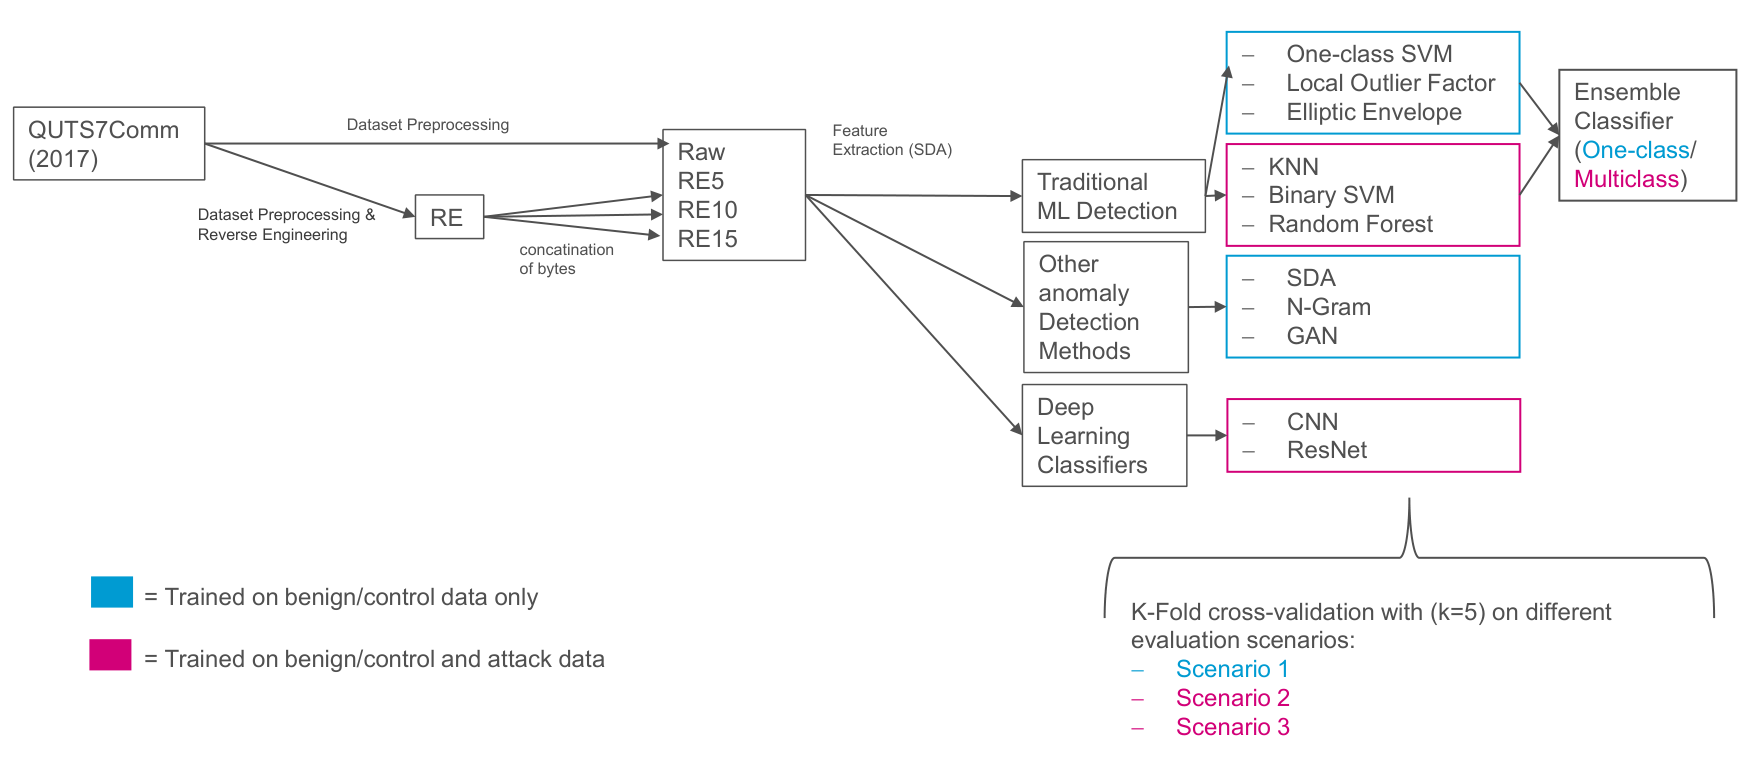
\includegraphics[width=\linewidth]{chapters/overview.png}
	\caption{Overview of proposed processing and evaluation pipeline}
 \label{fig:ourProcess}
\end{figure}

\Cref{fig:ourProcess} presents the complete processing pipeline of our
approach. The workflow begins with the provided \ac{pcap} files from the
2017QUTS7comm dataset. These packet captures are transformed and
preprocessed using two alternative strategies.

The first strategy operates directly on the raw packet data
(\textit{RAW} representation). The second strategy applies a
reverse-engineering procedure to extract a dynamic payload region,
which is assumed to contain process-related information.
After extraction, consecutive payload segments are concatenated
according to a parameter $p$, which controls the number of packets
aggregated into a single sample.

As a result, four dataset representations are generated:
\begin{itemize}
    \item \textbf{RAW}: processed packet data without reverse engineering,
    \item \textbf{RE5}, \textbf{RE10}, and \textbf{RE15}: reverse-engineered
    representations using $p \in \{5,10,15\}$, respectively.
\end{itemize}

Next, a \ac{SDA} is used to extract a compact latent feature vector
from each representation. These feature vectors serve as input for
the traditional \ac{ML} and selected \ac{DL} models.

The detection problem is considered from two perspectives:
outlier detection and supervised classification.
Accordingly, both one-class and supervised classifiers are evaluated.

We employ six traditional \ac{ML} models:

\begin{itemize}
    \item \textbf{One-class models:}
    \begin{itemize}
        \item One-Class \ac{SVM}
        \item \ac{LOF}
        \item \ac{EE}
    \end{itemize}
    
    \item \textbf{Supervised models:}
    \begin{itemize}
        \item Binary \ac{SVM}
        \item \ac{KNN}
        \item Random Forest
    \end{itemize}
\end{itemize}

In addition, two \ac{DL} classifiers are investigated:

\begin{itemize}
    \item \ac{CNN}
    \item \ac{ResNet}
\end{itemize}

Finally, three additional anomaly detection approaches are evaluated:

\begin{itemize}
    \item Reconstruction-error-based \ac{SDA}
    \item N-gram model
    \item \ac{GANs}-based detection
\end{itemize}

All detection methods are evaluated under three predefined
evaluation scenarios using $k$-fold cross-validation.

%%{\color{red} Due to limitation of our dataset size,} we needed to perform k-folding, however we considered performing the k-folding with three different scenarios. And for our whole experiments we considered the value of k to be equal to 5.  



\section{Dataset Pre-processing}

During the preprocessing we transform the provided PCAP files into
structured datasets suitable for training and evaluating the detection
methods. The process consists of label extraction, metadata parsing,
and the construction of two different dataset representations: RAW
and \ac{RE}.

%labe extraction
Attack labels were derived from the dataset folder structure.
Each PCAP file corresponds to either benign traffic or a specific
attack type, which allows assigning ground-truth labels to all
contained packets.
For every packet, we extracted relevant metadata including timestamps,
source and destination \ac{IP} addresses, and source and destination
port numbers. This metadata was used for filtering and dataset
organization but was not directly provided as input to the detection
models.

%raw ds representation

For the RAW representation, all packets contained in the PCAP files
were included without protocol-level filtering. This includes packets
without application-layer payload as well as packets unrelated to
the S7 communication protocol.

Each packet was represented by its complete raw byte sequence,
including Ethernet, \ac{IP}, and \ac{TCP}/\ac{UDP} headers followed by the
application-layer payload (if present). No additional parsing or
content truncation was performed in this representation.

%re dataset representaion

For the \ac{RE} representation, only S7Comm-related
application-layer data was considered. Packets were filtered according
to the following criteria:

\begin{itemize}
    \item The packet contains a \ac{TCP} layer,
    \item Either the source or destination port equals 102 (standard S7Comm port),
    \item The packet length satisfies the minimum structural size of
          TPKT (4 bytes), COTP (3 bytes), and S7 header (12 bytes).
\end{itemize}

After identifying valid S7Comm packets, only the application-layer
payload was retained. Based on the keyword position determined during
the reverse engineering phase, the byte sequence was truncated such
that only the payload starting from the identified keyword was used.
The keyword is identified in the Reverse Engineering process, as we describe in the following \cref{sec:rev-eng}. 
This representation therefore focuses on protocol-relevant content
rather than the full packet structure.

\subsection{Concatenation of Bytes to create RE5,RE10,RE15}

After identifying the index of the most suitable candidate keyword, we focused on extracting only the physical reading from the packets. However, we observed that extracting the physical reading from each packet individually results in very short byte sequences, which may not provide sufficient information for effective analysis. 

To address this limitation, we introduced a parameter denoted as \textit{p}, which defines the number of consecutive packets to be combined together. As illustrated in figure \ref{fig:ConcatenationOfBytes}, we concatenate the physical readings - which are located directly after the index of the best candidate - of every p consecutive raw packets to construct a single sample in the \ac{RE} dataset. 

More specifically, the physical readings extracted from raw packets $p_1$, $p_2$, ..., $p_p$ are concatenated to form single \ac{RE} sample. This process is repeated sequentially over the entire raw dataset. If the total number of raw packets is not divisible by p, the remaining packets at the end of the dataset are concatenated together without further padding or duplication. This concatenation strategy enables us to achieve three main objectives. First, it allows us to focus exclusively on the physical readings as features, thereby eliminating irrelevant protocol-related bytes from the analysis. Second, by combining consecutive packets, we partially reconstruct the contextual and temporal relationship between physical readings, which may improve the representational quality of the data. Finally, it allows us to systematically evaluate the impact of varying the parameter \textit{p} on the performance of the different detection methods. 



\begin{figure}[h]
    \centering
    \includesvg[width=0.8\textwidth]{Imgs/Concatenation}
    \caption{Concatenation of Bytes}
    \label{fig:ConcatenationOfBytes}
\end{figure}



\section{Reverse engineering}
\label{sec:rev-eng}
The objective of the reverse engineering process is to identify the
byte position (keyword) after which physical process readings are most
likely contained within the S7 communication payload. Since the protocol
specification is not explicitly parsed, the goal is to infer structural
patterns directly from the observed traffic.

\subsection{Identifying Keyword Candidates}

Firstly we identify all possible keyword candidates, by applying the following processing steps on the network traffic packets from the raw pcap files. 

\textbf{Session Extraction}

The network traffic is divided into communication sessions.
Sessions are identified based on the tuple
(source \ac{IP}, destination \ac{IP}, source port, destination port)
combined with a time window derived from packet inter-arrival times.
This grouping separates independent communication instances and
also distinguishes between client-to-server and server-to-client
directions.

\textbf{Progressive Sequence Alignment}

For each session and communication direction, progressive sequence
alignment is performed over all communication sessions. The purpose of
this alignment is to identify recurring structural patterns across
multiple messages.

\textbf{Identification of Static and Dynamic Fields}

Based on the aligned sequences, byte positions are classified as
\emph{static} if they remain constant across messages and as
\emph{dynamic} if their values vary.

Static byte positions typically correspond to protocol headers,
control fields, or structural identifiers, while dynamic positions
are potential candidates for variable data such as physical readings.
Adjacent static byte positions are merged into static fields to
form coherent structural blocks.

\textbf{Clustering of Dynamic Fields}

After separating static and dynamic fields, each dynamic field is
considered as a potential keyword candidate. For each candidate,
the subsequent payload region (i.e., the remaining frame behind the
candidate position) is extracted and grouped into value-based clusters.
The clustering is performed by grouping aligned
messages according to the byte values of the candidate field: messages with identical values
in the candidate interval $[start,end]$ are assigned to the same cluster.

The intuition is that if a candidate position marks the beginning
of physical readings, the subsequent byte sequences should exhibit
consistent value patterns across similar operational states.

\subsection{Cluster-Similarity Analysis for Keyword Selection}


After generating value-based clusters for each keyword candidate field, we analyze the
resulting cluster structure to identify the best keyword candidate.
For this we used the following approaches.
 

\subsubsection{Payload-Length Homogeneity within Clusters}
In addition to cluster-size statistics, we analyze whether messages grouped by a keyword
candidate exhibit consistent payload characteristics. For each aligned message, we compute its
effective payload length as the number of non-empty bytes (non-\texttt{None} positions) in the
alignment. For each cluster with at least two messages, we compute the standard deviation of
these payload lengths and aggregate the values across clusters using a size-weighted average.
A low homogeneity score indicates that messages within the same cluster have similar payload
lengths, which is expected when the candidate field groups messages into structurally similar
types. Candidates achieving low within-cluster variability are therefore considered more likely
to mark a meaningful boundary in the protocol payload.
\subsubsection{Joint Probability}

Not every candidate keyword identified during the previous steps represents a valid protocol keyword. Therefore, we introduce several constraints in order to filter out unlikely candidates. 

First, we define a maximum keyword length constraint. This constraint introduces a parameter \textit{L}, which represents the maximum allowed length of a keyword. Length of a keyword is defined as the number of bytes in the keyword. Any candidate keyword whose length exceeds \textit{L} is discarded. This step reduces the number of potential candidates and removes fields that are unlikely to represent protocol keywords.

For the remaining candidates, we evaluate the quality of the clustering results by computing three probability measures. These probabilities assess different structural and behavioral properties of the clusters and help determine the most likely keyword candidate.

\begin{itemize}

\item \textbf{Message Similarity ($P_m$):}  
This probability measures the similarity between messages within and across clusters. The underlying assumption is that messages belonging to the same cluster should exhibit higher similarity than messages belonging to different clusters.

For every pair of messages, we compute a similarity score defined as the ratio between the number of identical bytes and the total number of bytes in both messages. These scores form a similarity matrix containing the similarity values for all message pairs.

Based on the clustering results for a given keyword candidate, the similarity scores are divided into two groups:
\begin{itemize}
\item \textit{Intra-scores}: similarity scores between messages belonging to the same cluster.
\item \textit{Inter-scores}: similarity scores between messages belonging to different clusters.
\end{itemize}

A threshold parameter \textit{T} is then introduced in order to compute two additional metrics:

\begin{itemize}
\item \ac{FMR}:
\[
FMR = \frac{\#(\text{inter-scores} > T)}{\text{total number of inter-scores}}
\]

\item \ac{FNMR}:
\[
FNMR = \frac{\#(\text{intra-scores} < T)}{\text{total number of intra-scores}}
\]
\end{itemize}

Using these values, the message similarity probability is defined as:

\[
P_m = 1 - \frac{FMR + FNMR}{2}
\]

A higher value of $P_m$ indicates that the candidate keyword produces clusters with high internal similarity and low similarity across clusters, which suggests a good keyword candidate.

\item \textbf{Remote Coupling ($P_r$):}  
This probability evaluates the relationship between clusters of client messages and clusters of server responses. The intuition behind this metric is that messages of the same type sent by a client should typically trigger similar responses from the server.

The computation proceeds as follows:

\begin{enumerate}
\item Client-to-server messages are clustered.
\item Server-to-client messages are clustered independently.
\item Messages are then paired according to their TCP session order.
\end{enumerate}

For each client cluster we define:
\begin{itemize}
\item $N$: the number of client messages in the cluster.
\item $M$: the largest number of corresponding server responses that belong to the same server cluster.
\end{itemize}

The remote coupling probability is then defined as:

\[
P_r = \frac{M}{N}
\]

A high value of $P_r$ indicates strong correspondence between client requests and server responses, suggesting that the candidate keyword correctly separates different message types.

\item \textbf{Structure Coherence ($P_s$):}  
This probability measures how consistent the internal structure of messages is within each cluster. The assumption is that messages of the same type should share a similar structural format.

For each cluster, the messages are aligned again and the number of alignment gaps introduced during this process is counted. The probability is then computed as:

\[
P_s = 1 - \frac{\text{average number of gaps}}{\text{aligned message length}}
\]

A higher value of $P_s$ indicates that messages within the cluster share a consistent structure, which supports the validity of the candidate keyword.

\end{itemize}

Finally, we compute the joint probability as

\[
P_t = P_m \cdot P_r \cdot P_s
\]

under the assumption that the three probabilities are independent. The resulting value represents the overall likelihood that a candidate field corresponds to a valid protocol keyword. Candidates with higher values of $P_t$ are therefore considered more likely to represent legitimate keywords. And best keyword should be teh one with the highest joint probability.

Following this scheme we managed to correctly detect the best keyword in protocol S7comm, and we identified the keyword index 12 as shown in figure \ref{fig:best_Candidate_S7comm}, which is \textit{Item count field}, after which we can find the physical readings.
\begin{figure}[htb]
	\centering
	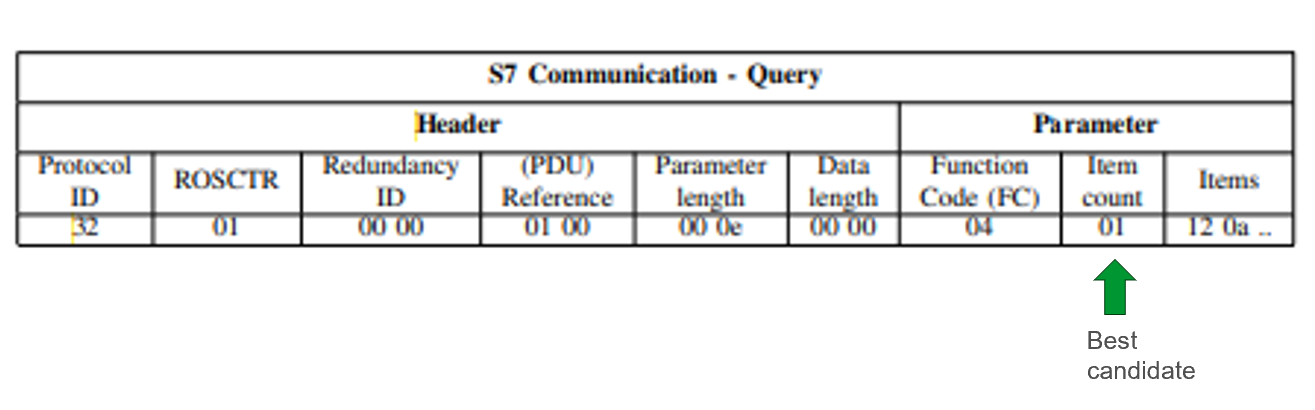
\includegraphics[width=\linewidth]{Imgs/S7comm_Best_Candidate.png}
    \caption{Determining best candidate index in S7comm protocol}
    \label{fig:best_Candidate_S7comm}
\end{figure}

\section{Evaluation Strategy}
To ensure a fair and systematic comparison of the implemented
detection methods, a structured evaluation strategy is adopted.
\subsection{Implementation of Evaluation Scenarios with K-Fold Cross-Validation}

Three evaluation scenarios are defined to simulate
different training conditions, ranging from purely benign
training data to partially supervised settings with varying
numbers of attack types.

\begin{itemize}
\item \textbf{Scenario 1:} The training set contains only benign samples.
\item \textbf{Scenario 2:} The training set contains all benign samples and
samples from $N-2$ of the $N$ attack types.
\item \textbf{Scenario 3:} The training set contains all benign samples and
samples from one randomly selected attack type.
\end{itemize}

In all scenarios, the test set contains benign samples as well as
samples from all attack types.

All scenarios are implemented using $k$-fold cross-validation with 5 iterations (k=5).

This method is used to obtain robust performance estimates by evaluating each model on multiple train-test splits. In addition, cross-validation makes efficient use of the available data, since every sample is used for validation exactly once and for training in the remaining folds.


\begin{figure}[htb]
	\centering
	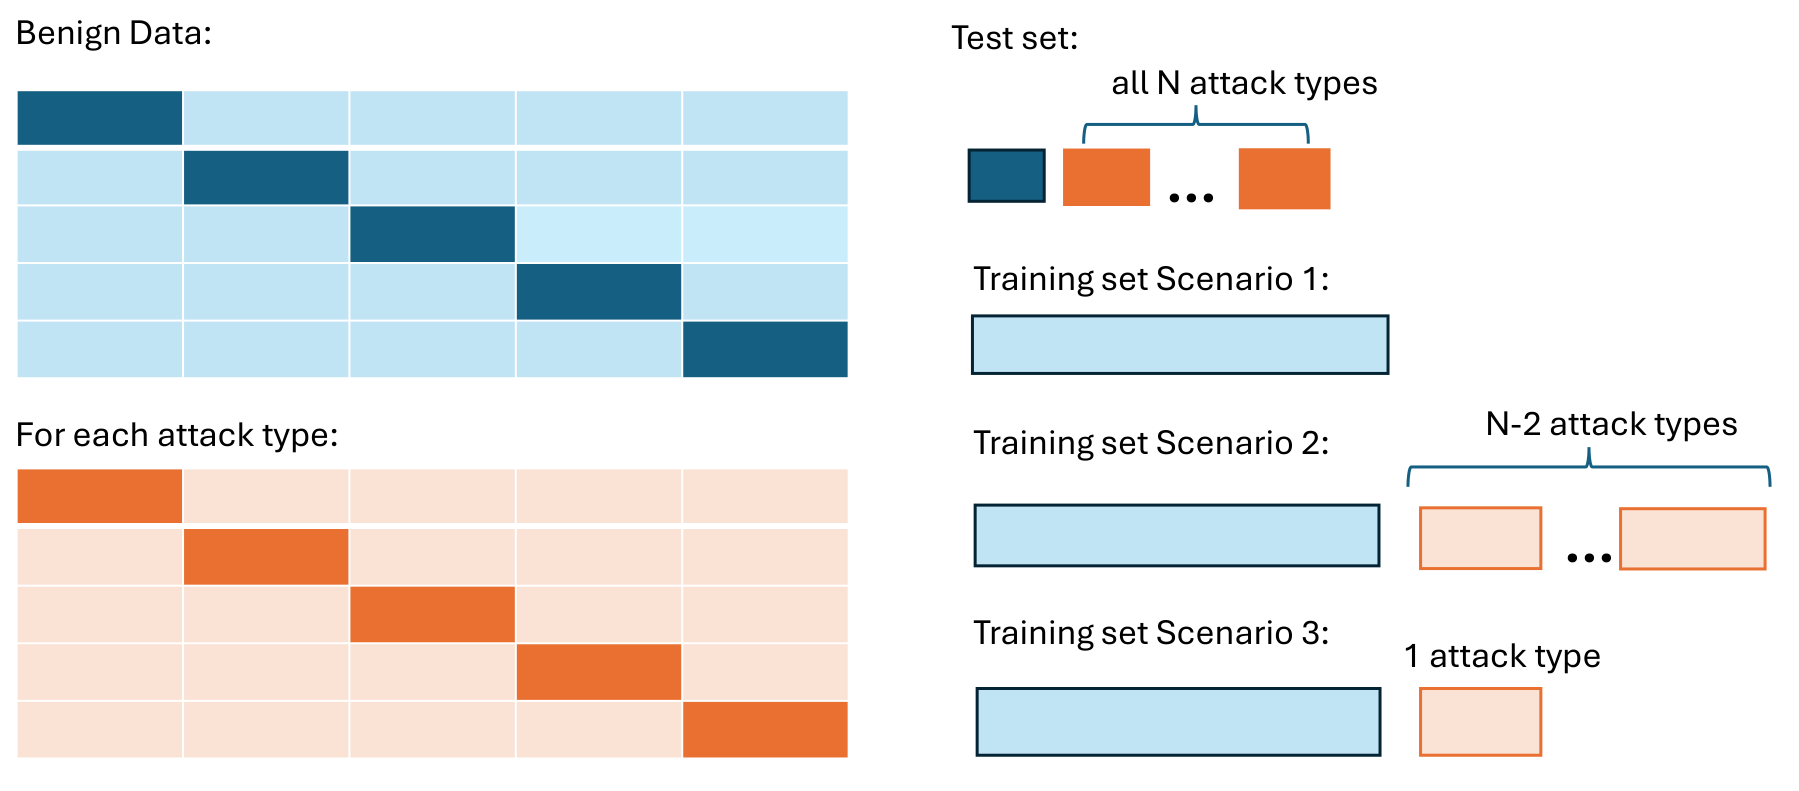
\includegraphics[width=\linewidth]{chapters/k_folds.png}
	\caption{K-Fold cross-validation adapted to the three evaluation scenarios}
	\label{fig:kfolds}
\end{figure}

To integrate the evaluation scenarios into the cross-validation
procedure, the dataset is first partitioned into benign samples
and separate subsets for each attack type.
Cross-validation is then performed independently on each subset.

As illustrated in figure \ref{fig:kfolds}, in each iteration the validation
fold of the benign subset is combined with the corresponding
validation fold of each attack-type subset to form the test split.
Consequently, the test split remains identical across all scenarios,
ensuring comparability between them.

The training split differs depending on the scenario:
\begin{itemize}
\item In \textbf{Scenario 1}, only the $k-1$ benign training folds are used.
\item In \textbf{Scenario 2}, the benign training folds are combined
with the $k-1$ training folds of $N-2$ attack types.
\item In \textbf{Scenario 3}, the benign training folds are combined
with the $k-1$ training folds of one randomly selected attack type.
\end{itemize}

As a result, the benign portion of the training data remains identical
across scenarios, while only the included attack types vary.
This design ensures that performance differences between scenarios
can be attributed to changes in attack diversity rather than
differences in test data.

\subsection{Evaluation Methods}

For each implemented model, hyperparameter tuning is performed
to determine optimal parameter configurations. It was usually performed using grid-search approach using the standard recommended values for each parameter.
Subsequently, experiments are conducted using these optimized
parameters within each fold and evaluation scenario.
Performance metrics are averaged across all cross-validation runs.

Since the test sets in all scenarios contain both benign and
attack samples and are not class-balanced, accuracy is not used
as the primary evaluation metric.
Instead, we report the F1-score,
which provides a more informative assessment under skewed
class distributions.

Beyond overall detection performance, we additionally analyze
feature importance, error overlaps, and computational complexity
(runtime and memory consumption) for the traditional ML classifiers.
These analyses are conducted for the RAW dataset representation
and for the RE15 representation to enable a detailed comparison
of classifier behavior under full and reduced feature sets.
%Feature Importance
\subsubsection{Feature Importance Analysis}
\label{subsubsec:feature_importance}

To better understand the contribution of the extracted features to the classification
decision, we perform a feature importance analysis for the traditional machine learning
classifiers. Since different models provide different interpretability mechanisms,
model-specific importance measures are used.

For the binary linear \ac{SVM}, feature importance is computed
as the absolute magnitude of the learned weight vector, i.e., $|\mathbf{w}|$,
which reflects the contribution strength of each input feature to the decision boundary.

For the Random Forest classifier, we use the built-in impurity-based importance
measure (mean decrease in impurity), which quantifies how much each feature
contributes to reducing node impurity across all trees in the ensemble.

For all other traditional \ac{ML} classifiers, permutation-based feature importance
is applied. In this approach, the values of a single feature are randomly permuted,
and the decrease in model performance is measured. A larger performance drop
indicates higher feature relevance.

The resulting importance scores are normalized and ranked in descending order.
This analysis allows us to identify which autoencoder-generated features contribute
most to attack detection and to compare feature reliance across different models.

%Venn Diagrams for Error Overlaps
\subsubsection{Error Overlap Analysis}

To analyze the overlap of classification errors among different detection methods,
we construct Venn diagrams for each evaluation scenario. Each circle represents the set
of misclassified test samples produced by a particular classifier. Intersections between
circles indicate samples that were misclassified by multiple models simultaneously.

This analysis provides insight into whether different classifiers fail on the same
instances or whether their errors are complementary. A high degree of overlap suggests
that the models capture similar patterns, whereas low overlap indicates complementary
behavior.

%Runtime and Memory consumtion
\subsubsection{Runtime and Memory Consumption}

In addition to detection performance, we evaluate the computational complexity of
each method in terms of runtime and memory consumption. For each model, we measure:

\begin{itemize}
    \item Feature generation time, measured separately for (i) training the autoencoder and (ii) extracting features from the trained model
    \item Average training time and average inference time for each traditional \ac{ML} detection method,
    \item Peak memory usage during feature generation,  measured separately for (i) training the autoencoder and (ii) extracting features from the trained model
    \item Peak memory usage during training and inference for each traditional ML detection method.
\end{itemize}

Runtime is measured using system time functions, while memory consumption is monitored
using profiling tools. The reported values correspond to the average across all
cross-validation folds.

This analysis allows us to compare the practical feasibility of traditional machine
learning methods.

\section{Implementation of Anomaly detection methods}

This subsection describes the traditional machine learning methods used for anomaly detection. 
First, we explain how latent features are extracted from the packet data using the \ac{SDA}. These features are then used as input to our classifiers implemented in our framework.

\subsection{Traditional \ac{ML} detection methods}


To apply traditional machine learning classifiers to network packet data, a fixed-length feature 
representation is required. Therefore, we first extract compact latent representations from the 
raw packet data using the \ac{SDA}.


%ToDo Anna
\subsubsection{Feature Extraction using the \ac{SDA}}
Traditional ML classifiers such as \ac{SVM}, \ac{KNN}, and Random Forest require a fixed-length, low-dimensional feature representation and do not natively handle variable-length byte sequences. Therefore we employ a \ac{SDA} as a feature extractor to obtain compact latent representations of the preprocessed
packet data. These latent feature vectors are subsequently used as input to all traditional
machine learning detection methods.

Each sample in a dataset representation (RAW, RE5, RE10, RE15) is given as a byte-vector.
To ensure a fixed input dimensionality, every byte-vector is either truncated or zero-padded
to a predefined length $M$ and then normalized to the range $[0,1]$. In our experiments,
$M$ was set to the length of the longest packet (or concatenated RE sequence) within the
corresponding representation.
For each dataset representation, the \ac{SDA} is trained exclusively on benign samples and on the training set from the current k-fold iteration. Using only benign samples enables the
model to learn a compressed representation of normal traffic patterns.

After training, the \ac{SDA} is used to encode all samples of the corresponding representation.
Concretely, each input byte-vector is forwarded through the encoder, and the output vector of
the bottleneck layer are extracted as the latent feature vector. In our implementation, the
bottleneck produces a 32-dimensional feature vector per input sample, resulting in a compact
representation that is used for subsequent training and evaluation of the traditional ML
classifiers.

\subsubsection{Ensemble Classifier Implementation}

\begin{figure}[htb]
	\centering
	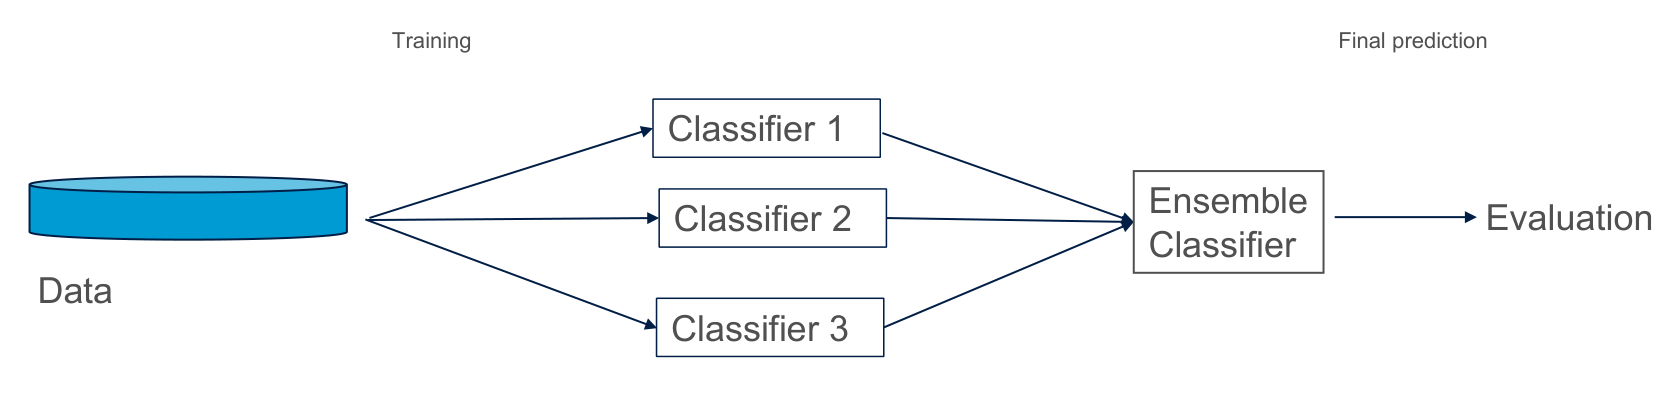
\includegraphics[width=\linewidth]{chapters/ensembleClassifier.png}
	\caption{Ensemble Classifier Structure}
 	\label{fig:ensemble-structure}
\end{figure}
In order to reduce model-specific errors and leverage complementary strengths to achieve an overall more robust and stable detection performance we combine the traditional ML classifiers into an ensemble classifier. 

As illustrated in figure \ref{fig:ensemble-structure} the ensemble classifier combines the predictions of three independently
trained traditional machine learning models.
 Each base classifier is
trained separately using the corresponding training split of the
cross-validation procedure. During inference, all three classifiers
produce an individual prediction for each test instance.

The final decision of the ensemble is obtained by aggregating the
three individual predictions according to a predefined aggregation
strategy. In our implementation, the following prediction modes are
supported:

\begin{itemize}
    \item \textbf{Random:} One of the three predictions is selected uniformly at random.
    \item \textbf{Majority:} The final prediction corresponds to the class predicted by the majority of the three classifiers.
    \item \textbf{All:} A sample is classified as an attack only if all three classifiers predict it as an attack; otherwise, it is classified as benign.
\end{itemize}

Since the project includes six traditional ML detection methods: three
operating as one-class (outlier) detectors and three operating as
binary classifiers—we implemented two operational ensemble modes:

\begin{itemize}
    \item \textbf{One-Class Mode:} The ensemble aggregates the predictions of the three outlier detectors (One-Class SVM, LOF, and Elliptic Envelope).
    \item \textbf{Binary Classification Mode:} The ensemble aggregates the predictions of the three binary classifiers (Binary SVM, k-Nearest Neighbors, and Random Forest).
\end{itemize}

\subsection{\ac{DL} detection methods}


In addition to traditional machine learning approaches, we implement deep learning based
detection methods that can learn hierarchical feature representations directly from the
raw byte sequences of network packets. Unlike traditional classifiers, deep neural networks
can automatically capture complex spatial patterns and dependencies in packet data without
relying on manually engineered features.

In particular, we investigate \ac{CNN} and \ac{ResNet}. \ac{CNN}s are well suited for analyzing structured sequential data such as byte
sequences, as convolutional filters can learn local patterns that frequently occur in
network packets. \ac{ResNet} extends this idea by introducing residual connections that allow
training deeper neural architectures while mitigating the vanishing gradient problem.
These models enable the system to learn more expressive representations of the packet
structure and improve anomaly detection performance.

\subsubsection{\ac{CNN}}
%ToDo Anna

We implemented a \ac{CNN} to perform binary attack detection directly on the preprocessed byte sequences (i.e., without using the autoencoder-generated features). Similar to the feature generation pipeline, all
inputs are converted to a fixed length of $M$ bytes by truncation or zero-padding to ensure a
consistent input shape. For our experiments, $M$ was set to the length of the longest packet
in the corresponding dataset representation. Each sample is provided to the network in the
shape $(M,1)$, where the last dimension represents the single input channel.

The CNN consists of four convolutional blocks followed by a dense classification head.
Each convolutional block contains two repetitions of the sequence
\emph{Conv1D $\rightarrow$ Batch Normalization $\rightarrow$ Activation $\rightarrow$ Dropout}.
The convolution layers learn local byte-patterns by applying trainable filters across the input
sequence, batch normalization stabilizes training by normalizing intermediate activations, and
dropout reduces overfitting by randomly deactivating a fraction of units during training.
The number of filters increases with network depth (e.g., $8,16,32,64$), enabling the model to
learn progressively more abstract representations.

To reduce the temporal resolution between blocks, we apply downsampling either via
MaxPooling1D after each block or by using stride-2 in the first convolution of blocks two to
four (depending on the selected configuration). After the fourth block, the resulting feature
maps are transformed into a fixed-size vector using a global pooling operation.
By default, we apply Global Average Pooling, which aggregates each feature map by averaging
over its length dimension and produces a compact representation for the dense layers.

Finally, the network applies a fully connected layer (with batch normalization, activation, and
dropout) and a Softmax output layer with two neurons to predict the probability of the classes
\emph{benign} and \emph{attack}. The model is optimized using Adam and categorical cross-entropy
loss. Architecture-related hyperparameters (e.g., activation function, kernel size, dropout rate,
downsampling strategy, and pooling type) as well as optimization parameters were selected via
grid search on the training split.

\subsubsection{\ac{ResNet}} 
 In the context of anomaly detection in \ac{ICS}, ResNet can be adapted to process one-dimensional byte sequences of network packets using one-dimensional convolutional layers. The residual connections help preserve low-level structural information while progressively extracting higher-level representations, which improves classification performance on complex and high-dimensional network traffic data. Due to its stable training behavior and strong representational capacity, ResNet is particularly suitable for modeling subtle deviations in proprietary binary communication protocols. ResNet accepts as an input \textit{m} x \textit{n} complete network packets or the parsed physical readings, where m is the number of packets, and n is the number of bytes per each packet. 


\begin{figure}[h]
    \centering
    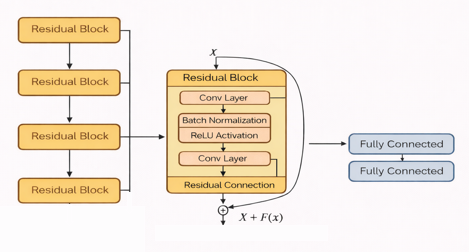
\includegraphics[width=1.0\textwidth]{Imgs/ResNetArch.jpg}
    \caption{ResNet18 Architecture}
    \label{fig:resNetArch}
\end{figure}

\vspace{10px}


\paragraph{Our implementation} We managed to implement ResNet18 which contains of 18 layers in total.  these layers are divided into four main residual blocks as shown in figure \ref{fig:resNetArch} and each block consists of two convolution blocks. Each convolution block contains two convolution layers with a batch normalzation and ReLU non-linear activation function in between. After the 4 residual blocks, we forward the output to two fully-connected layers, that will use the reduced data to classify the network packet using sigmoid function. We used Adam optimizer to update weights, and for the loss function we used categorical cross-entropy. 
\paragraph{Statistical features} Along with the raw network packets, and the reverse engineered packets, we managed to extract 5 other statistical features and append them to the ResNet. 

\begin{enumerate}
    \item Total number of bytes in a given sample packet which is counted before trimming or padding this packet.
 \item Number of occurrence of the most often found byte
 \item Number of occurrence of the second most often found byte,
 \item Byte entropy, which measures randomness of packet bytes. It is computed as \[
E(P) = - \sum_{b=0}^{255} p(b)\,\log_2 p(b)
\] 
where $p(b)$ denotes the probability of observing byte value $b$ in the packet.
\[
p(b) = \frac{n_b}{N}
\]
where ${n_b}$ is number of  occurrences of byte b in the given packet, and N is the size of the packet. 
 \item \ac{RPB}, which tells the model how much of the input is artificial. It is computed as \[
\mathrm{RPB} = \frac{\text{number of bytes before padding}}{\text{total number of bytes}}
\]
\end{enumerate}

\subsection{Other anomaly detection methods}

In addition to the traditional ML and deep learning classifiers, we evaluate several alternative
approaches for anomaly detection. These include an SDA-based reconstruction error detector,
an n-gram statistical model that captures byte sequence patterns in network packets, and a
\ac{GANs} based method capable of modeling the distribution of
normal traffic. These methods provide complementary perspectives on anomaly detection by
leveraging reconstruction errors, statistical sequence modeling, and generative learning.

\begin{figure}[htb]
	\centering
	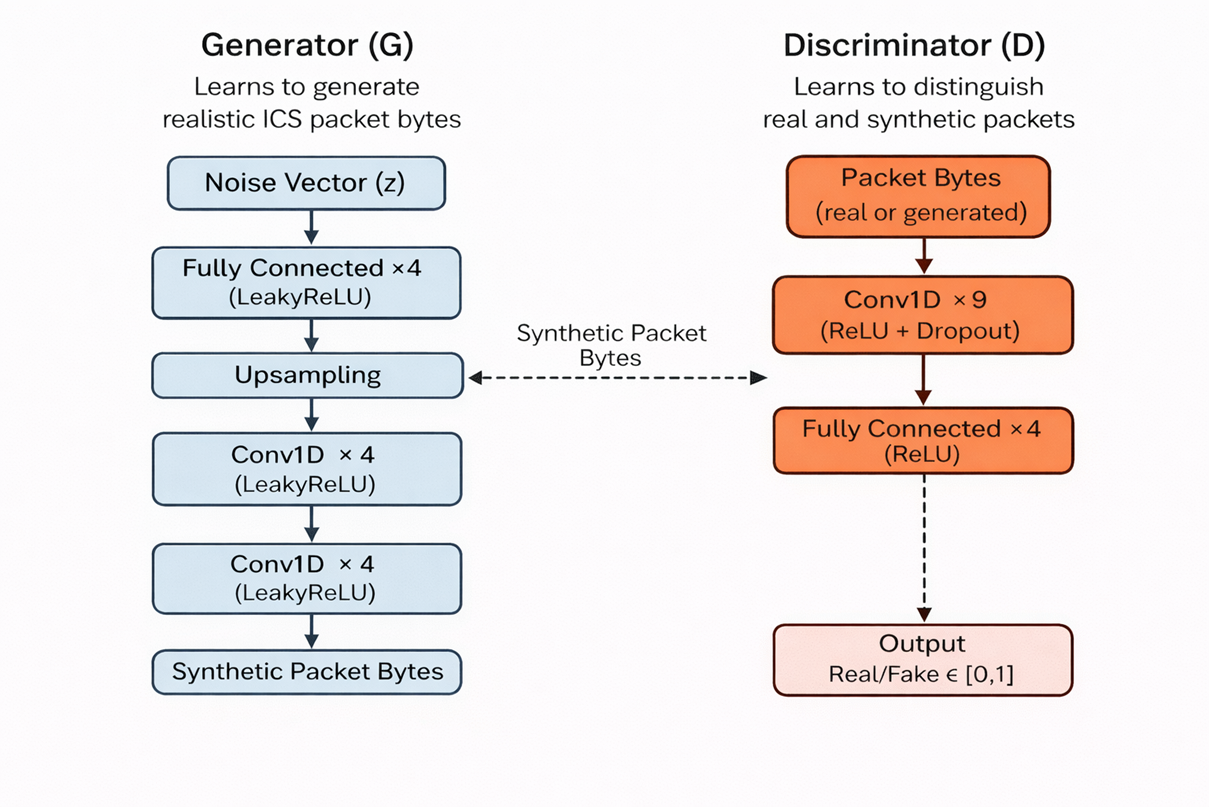
\includegraphics[width=\linewidth]{Imgs/Discriminator_and_Generator.png}
	\caption{Discriminator and Generator architectures}
    \label{fig:DandG}
\end{figure}


\subsubsection{\ac{SDA}-Based Reconstruction Error Detection}

The implemented \ac{SDA}
is employed as a standalone anomaly detection method based on
reconstruction error. The \ac{SDA} is trained exclusively on benign network traffic. During training,
the model learns a compressed latent representation of normal packets and
optimizes its parameters to minimize the reconstruction error between the
input and the reconstructed output. Since attack packets deviate from the
distribution of normal traffic, they are expected to be reconstructed less
accurately, resulting in a higher reconstruction error.

For a given input byte-vector $\mathbf{x} \in \mathbb{R}^M$, the trained
autoencoder produces a reconstruction $\hat{\mathbf{x}}$. The reconstruction
error is computed using the \ac{MSE}:

\begin{equation}
\text{MSE}(\mathbf{x}) = \frac{1}{M} \sum_{i=1}^{M} (x_i - \hat{x}_i)^2.
\end{equation}

To transform the \ac{SDA} into a binary classifier, a decision threshold
$\tau$ is defined based on the reconstruction error distribution of
benign training samples. Concretely, we compute the per-sample \ac{MSE}
for all benign training packets and set $\tau$ to the
$95^{\text{th}}$ percentile of these errors, i.e., such that
95\% of benign reconstruction errors lie below $\tau$.

During testing, each packet is processed by the trained \ac{SDA} and its
reconstruction error is computed. The final classification rule is:

\begin{equation}
\hat{y} =
\begin{cases}
\text{attack}, & \text{if } \text{MSE}(\mathbf{x}) > \tau, \\
\text{benign}, & \text{otherwise}.
\end{cases}
\end{equation}

Packets whose reconstruction error exceeds the predefined threshold
are therefore classified as anomalous.


\subsubsection{\ac{GANs}}
In anomaly detection scenarios, particularly in \ac{ICS}, GANs can be trained on normal data only, allowing the discriminator or generator to detect deviations from the learned distribution during testing. Because GANs are capable of learning complex, high-dimensional data distributions, they are well suited for modeling raw network packet bytes or other structured sequential inputs. 




\paragraph{Discriminator Implementation}
 
 Discriminator architecture as shown in figure \ref{fig:DandG} consists of \ac{CNN} that consists of 9 convolution layers with ReLU activation function, along with dropout layer after all convolution layers except the first and final layers. Output is passed to four fully connected layers with ReLU activation function, and the output is generated from Sigmoid function which predicts a value in range [0,1] indicating how fake the input data is, 0 means fake data, while 1 means real data. 

\paragraph{Generator Implementation} Generator is reverse \ac{CNN}. It uses \textit{deconvolution} operation, which is he inverse operation of convolution, which is a method to transform noise into meaningful network packets with a certain degree of accuracy. Its architecture as shown in figure \ref{fig:DandG}  consists of 4 fully connected layers with a LeakyReLU activation function, then they are followed by 8 convolution layers with LeakyReLU activation function. The first 4 layers from these 8 convolution layers are preceded by upsampling layers, the main reason for that is to increase the number of data samples in the dataset, which can helps in correcting imbalances in data, enhancing the quality of generated data, and improve the model performance.  We mainly used LeakyReLU here because we want to be able to regenerate the network packet out of noise input, so it can help us keeping as much neurons alive as possible to participate in the generation of the network packets. Moreover, for the generator we managed to implement custom loss function, which extract features from real and fake samples, and compute the mean feature vectors, then it computes L2 loss between mean feature vectors. \begin{lstlisting}
def feature_matching_loss(D, x_real, x_fake):
    '''
    Input:
        D: Discriminator model
        x_real: real data batch
        x_fake: fake data batch
    Output:
        loss: feature matching loss value
    '''
    f_real = D.extract_features(x_real)
    f_fake = D.extract_features(x_fake)

    mean_real = f_real.mean(dim=0)
    mean_fake = f_fake.mean(dim=0)

    loss = torch.mean((mean_real - mean_fake) ** 2) / mean_real.numel()
    return loss
\end{lstlisting}



\subsubsection{N-Gram} 
It is a contiguous sequence of $N$ items extracted from a larger sequence of data, where the items may represent characters, bytes, or tokens depending on the application domain. In the context of network traffic analysis, N-grams are typically constructed from raw packet bytes, meaning that each N-gram represents a sequence of $N$ consecutive bytes within a packet. N-gram is usually defined by 2 main parameters, the value of \textit{n}, which defines the number of consecutive bytes, and \textit{stride} which define the jumping value. For example a 2-gram (bigram) with stride = 1  captures pairs of adjacent bytes, while a 5-gram with stride = 1 captures sequences of five consecutive bytes. In figure \ref{fig:n-gram-example}, we demonstrate the idea of n-grams but on string of characters, when n=3, and stride=1, we can see that we consider the first three consecutive characters \textit{HEL} as one feature, then we increase the pointer position by the stride value which is equal to 1 in our case to next starting position, and it will be in our case letter \textit{E}, then we take 3 consecutive characters again to form \textit{ELL}, and we keep this process till the end of the string. On the second example you can see the stride value is 2, so it will have the same behavior, except that when we go to the next starting index, instead of increasing the starting position by 1, we will increase it by 2, so in the second iteration instead of starting from index 1, we will start from 2 which contains letter \textit{L} instead of letter \textit{E}.  The main idea behind N-gram modeling is that local sequential patterns contain meaningful structural information about the underlying data distribution. During the training phase, all distinct N-grams observed in benign traffic are collected and their frequencies are recorded, often using memory-efficient data structures such as \textbf{Bloom filters}. At testing time, a new packet is evaluated by measuring how many of its N-grams were previously observed during training and how frequently they occurred. We define a score for whether this packet is normal or malicious as: \[
\text{Score} = \frac{\sum_{i} w_i \cdot N_{\text{seen}_i}}{T}
\] 
$\text{Score} \in [0,1]$, where $N_{\text{seen}_i}$
indicates each n-gram in the packet that was seen during training,
wi represents its normalized weight how often this n-gram was seen during training, and T
represents the total number of n-grams in the current packet. Packets that contain a high proportion of unseen or rarely occurring N-grams are more likely to deviate from normal behavior and can therefore be classified as anomalous, in other words, packets with low scores should be classified as malicious. N-gram-based methods are particularly suitable for anomaly detection in \ac{ICS} because proprietary binary protocols often lack publicly available specifications, making direct parsing difficult. By operating directly on raw byte sequences without requiring protocol awareness, N-grams provide a simple yet effective statistical modeling technique for detecting deviations in structured network traffic. \paragraph{Bloom Filter} is a probabilistic data structure designed for efficient set membership testing with minimal memory consumption. It allows one to determine whether an element is possibly in a set or definitely not in a set. A Bloom filter consists of a fixed-size bit array and multiple independent hash functions. When inserting an element into the filter, the element is processed by each hash function, and the corresponding bit positions in the array are set to one. To check whether an element is present, the same hash functions are applied, and the bits at the resulting positions are inspected. If at least one of these bits is zero, the element is guaranteed not to be in the set. If all bits are one, the element is assumed to be in the set; however, this may result in a false positive due to hash collisions. Importantly, Bloom filters do not produce false negatives, meaning that an inserted element will never be reported as absent. The trade-off between memory usage and false positive probability depends on the size of the bit array and the number of hash functions used. In the context of N-gram-based anomaly detection for \ac{ICS}, Bloom filters are particularly useful for storing large numbers of observed N-grams in a space-efficient manner, enabling fast membership queries during testing without requiring storage of the full set of N-grams.

\begin{figure}[htb]
	\centering
	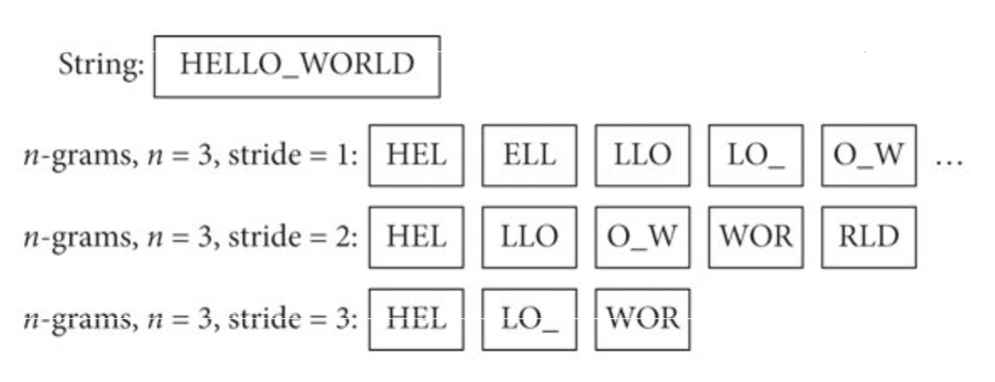
\includegraphics[width=\linewidth]{Imgs/n_grams_example.png}
	\caption{N-Gram Example}
	\label{fig:n-gram-example}
\end{figure}


\paragraph{Hash Functions and Double Hashing Strategy}


Instead of computing $k$ independent hash functions, we apply a double hashing strategy. 
Two base hash values $h_1(x)$ and $h_2(x)$ are computed, and the $i$-th hash value is generated as:

\[
h_i(x) = \left(h_1(x) + i \cdot h_2(x)\right) \bmod m
\]

where $m$ denotes the size of the Bloom filter in bits.

This approach significantly reduces computational cost while maintaining good distribution 
properties and minimizing correlations between generated hash values. For h1 and h2 we used both a non-cryptographic and a cryptographic hash function to ensure a good balance between speed and randomness, which are MurmurHash3 and BLAKE2b respectively.

\textbf{MurmurHash3} is a non-cryptographic hash function optimized for high speed and low computational overhead. 
It produces a uniform 64-bit output and is widely used in Bloom filters and hash tables due to its strong 
avalanche effect and low collision probability in practical applications.

\medskip

\textbf{BLAKE2b} is a cryptographic hash function designed to provide both high security and high performance. 
It generates outputs with strong entropy and collision resistance. 
In our implementation, we use an 8-byte (64-bit) digest to obtain a compact yet well-distributed hash value.



\begin{lstlisting}
def _hashes(self, data: bytes):
    '''
    Generate k hash values for the given data using double hashing.
    Parameters:
        data: byte sequence to be hashed

    Yields:
        k hash values in the range [0, m-1]
    '''

    # First hash: MurmurHash3 (fast, non-cryptographic)
    h1, _ = mmh3.hash64(data, seed=0, signed=False)

    # Second hash: BLAKE2b (cryptographic, strong entropy)
    blake = hashlib.blake2b(data, digest_size=8).digest()
    h2 = int.from_bytes(blake, "big") | 1  # ensure h2 is odd

    # Generate k hash values using double hashing
    for i in range(self.number_of_hash_functions):
        yield (h1 + i * h2) % self.required_number_of_bits
\end{lstlisting}


